\documentclass[10pt]{article}
\usepackage[margin=0.8in]{geometry}
\usepackage{booktabs}
\usepackage{microtype}
\usepackage{pgfplots}
\pgfplotsset{compat=1.18}
\begin{document}
\section*{DOOM Quality Modernization: Before vs. After}
This report contains aggregate measurements only. Individual diagnostic paths and messages are intentionally excluded so report size does not scale with finding count.

Before corpus: \texttt{doom}.\\
After corpus: \texttt{interop/algorithms/quality/in/doom}.\\
Pinned validator toolchain: LLVM/Clang 22.1.8.
\subsection*{Corpus metrics}
\begin{tabular}{lrr}
\toprule Metric & Before & After \\
\midrule
C translation units & 72 & 62 \\
Headers & 74 & 64 \\
Physical source lines & 59110 & 50851 \\
Nonblank source lines & 48963 & 44026 \\
Source bytes & 1333724 & 1497009 \\
Local WAD files & 1 & 1 \\
Local WAD bytes & 28795076 & 28795076 \\
\bottomrule
\end{tabular}

WAD files are reported separately and are excluded from source LOC and source-byte measurements.
\subsection*{Quality outcome}
\begin{tabular}{lrrr}
\toprule Metric & Before & After & Reduction (\%) \\
\midrule
Unique findings & 143662 & 38462 & 73.23 \\
Raw reports & 201160 & 94085 & 53.23 \\
Findings / KLOC & 2430.42 & 756.37 & 68.88 \\
\bottomrule
\end{tabular}
\subsection*{Findings by gate}
\begin{tabular}{lrr}
\toprule Gate & Before & After \\
\midrule
clang-format & 75797 & 1 \\
clang-linux-arm64 & 3 & 1 \\
clang-linux-x86\_64 & 2497 & 861 \\
clang-tidy & 43619 & 37373 \\
editorconfig & 21720 & 222 \\
interop & 26 & 4 \\
\bottomrule
\end{tabular}
\subsection*{Findings by rule family}
\begin{tabular}{lrr}
\toprule Family & Before & After \\
\midrule
analyzer & 1 & 321 \\
bugprone & 540 & 381 \\
compiler & 4992 & 1723 \\
format & 75797 & 1 \\
hicpp & 1731 & 1553 \\
interop/other & 3488 & 2950 \\
misc & 2807 & 2350 \\
modernize & 1755 & 692 \\
performance & 26 & 5 \\
readability & 30805 & 28264 \\
text & 21720 & 222 \\
\bottomrule
\end{tabular}
\subsection*{Visual comparison}
\begin{center}
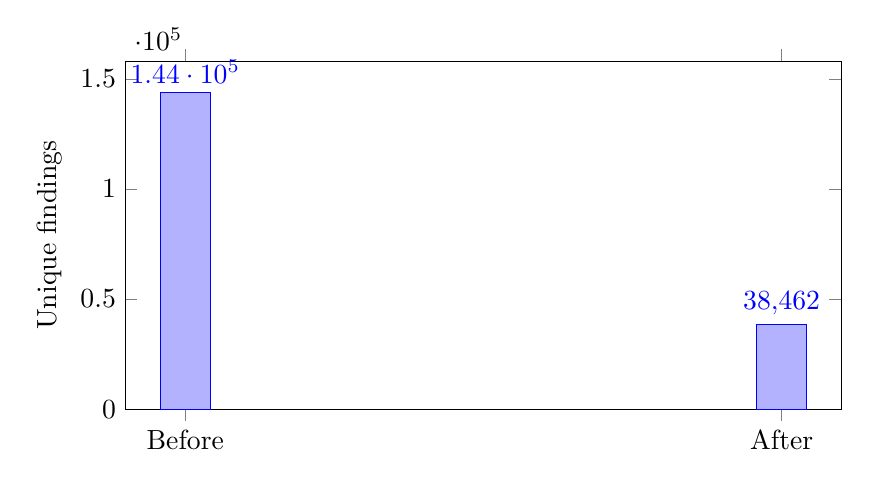
\begin{tikzpicture}
\begin{axis}[
ybar,
bar width=18pt,
width=0.88\linewidth,
height=6cm,
ylabel={Unique findings},
symbolic x coords={Before,After},
xtick=data,
nodes near coords,
ymin=0,
]
\addplot coordinates {(Before,143662) (After,38462)};
\end{axis}
\end{tikzpicture}
\end{center}
\subsection*{Reproducibility}
Before source SHA-256: \texttt{a7c20cd5bcdad32c87a85d855b2a77c63be5591ebf8186550436e75587d72ec7}.\\
After source SHA-256: \texttt{be5d56af7c2195582b004687a3dcab8d8e95295f636a75edf3f4dfc05096475f}.\\
Before asset SHA-256: \texttt{4c4be70ada080ac58c139e36c09b4ab89ff53bc06626fa3e417beffe39174711}.\\
After asset SHA-256: \texttt{4c4be70ada080ac58c139e36c09b4ab89ff53bc06626fa3e417beffe39174711}.\\
Machine-readable aggregate metrics: \texttt{interop/algorithms/quality/comparison/metrics.json}.
The generator intentionally stores no per-finding ledger.
\end{document}
